\documentclass[11pt]{beamer}
\usepackage[utf8x]{inputenc}

\definecolor{dredcolor}{rgb}{.9,0.2,0.2}


\mode<presentation>
{
  \setbeamercovered{transparent}
  \setbeamercolor{normal text}{fg=white,bg=gray}
  \setbeamercolor{alerted text}{fg=white}
  \setbeamercolor{example text}{fg=white}
  \setbeamercolor{background canvas}{bg=darkgray} 
  \setbeamercolor{structure}{fg=white}

  \setbeamercolor{block title}{bg=dredcolor,fg=white}
  \setbeamercolor{block body}{bg=white,fg=darkgray}

  \setbeamercolor{palette primary}{use=structure,fg=structure.fg}

  \setbeamercolor{math text}{}
  \setbeamercolor{math text inlined}{parent=math text}
  \setbeamercolor{math text displayed}{parent=math text}

  \setbeamercolor{normal text in math text}{}

  \setbeamercolor{local structure}{parent=structure}

  \setbeamercolor{titlelike}{parent=structure}

  \setbeamercolor{title}{parent=titlelike}
  \setbeamercolor{title in head/foot}{parent=palette quaternary}
  \setbeamercolor{title in sidebar}{parent=palette sidebar quaternary}

  \setbeamercolor{subtitle}{parent=title}
}

\usepackage{xspace}
\usepackage{graphicx}
\usepackage{tikz}

\def\hlt{\color{yellow}}

\usepackage{amsmath,amsfonts,amssymb,amsthm}
\usepackage[vlined,linesnumbered]{algorithm2e}

\newcommand{\field}[1]{\mathbb{#1}}
\newcommand{\F}{\ensuremath{\field{F}}\xspace}
\newcommand{\FZ}{\ensuremath{\field{F}_2}\xspace}
\newcommand{\FZE}{\ensuremath{\field{F}_{2^e}}\xspace}
\newcommand{\erange}{\ensuremath{2 \leq e \leq 10}\xspace}
\newcommand{\mzedt}{\texttt{mzed\_t}\xspace}
\newcommand{\mzdslicet}{\texttt{mzd\_slice\_t}\xspace}
\newcommand{\ord}[1]{\ensuremath{\mathcal{O}\!\left(#1\right)}}
\newcommand{\Magma}{\textsc{Magma}\xspace}
\newcommand{\PolyBoRi}{\textsc{PolyBoRi}\xspace}
\newcommand{\Sage}{Sage\xspace}
\newcommand{\GAP}{GAP\xspace}
\newcommand{\mycomputer}{2.66~Ghz Intel i7\xspace}

\newcommand{\memph}[1]{{\hlt{\bf #1}}}

\newtheorem{thm}{Theorem}[section]

\AtBeginSection[]
{
   \begin{frame}{Outline}
  \tableofcontents[currentsection]
  \begin{flushright}
  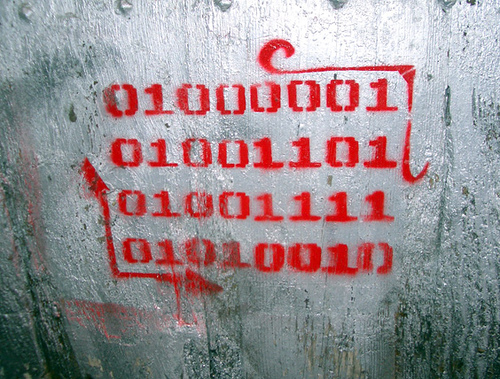
\includegraphics[height=0.2\textwidth]{gf2.jpg}
  \end{flushright}
  \end{frame}
}

\AtBeginSubsection[]
{
   \begin{frame}{Outline}
  \tableofcontents[currentsubsection]
  \begin{flushright}
  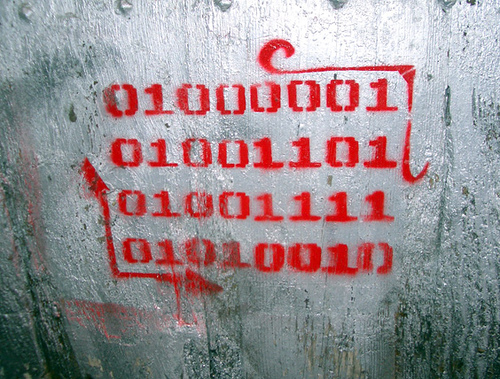
\includegraphics[height=0.2\textwidth]{gf2.jpg}
  \end{flushright}
  \end{frame}
}


\title{The M4RIE library for dense linear algebra over small fields with even characteristic}
\author{Martin R.\ Albrecht (martinralbrecht@googlemail.com)}
\institute{POLSYS Team, UPMC, Paris, France}
\date{ISSAC 2012, Grenoble, France}


\begin{document}

\begin{frame}
\titlepage
\end{frame}

\begin{frame}
\frametitle{Outline}
\tableofcontents
\begin{flushright}
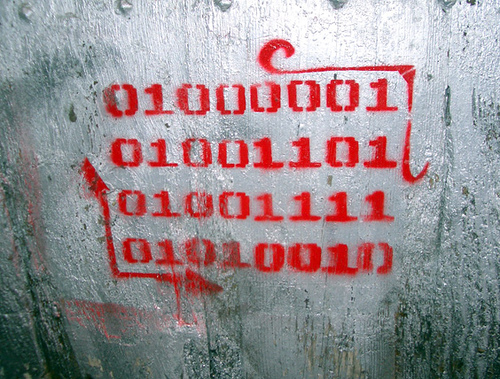
\includegraphics[height=0.2\textwidth]{gf2.jpg}
\end{flushright}
\end{frame}

\begin{frame}
\frametitle{The M4RIE Library}
\begin{itemize}
\item handles $\mathbb{F}_{2^e}$ for $2 \leq e \leq 10$; $e \leq 16$ planned.
\item available under the GPL Version 2 or later (GPLv2+)
\item provides basic arithmetic (addition, equality testing, stacking, augmenting, sub-matrices, randomisation, etc.)
\item implements asymptotically fast multiplication (this talk)
\item implements asymptotically fast elimination (this talk)
\item Linux, Mac OS X (x86 and PPC), OpenSolaris, and Windows (Cygwin)
\end{itemize}

\begin{block}{}
\centering
\url{http://m4ri.sagemath.org} 
\end{block}
\end{frame}

\begin{frame}[allowframebreaks]
\frametitle{Representation of Elements} 

Elements in $\F_{2^e} \cong \F_2[x]/f$ can be written as $$a_0 \alpha^0 + a_1 \alpha^1 + \dots + a_{e-1} \alpha^{e-1}.$$

\vspace{1em}

We identify the bitstring $a_0,\dots,a_{e-1}$ with
 \begin{itemize}
  \item the element $\sum_{i=0}^{e-1} a_i \alpha^i \in \F_{2^e}$ and
  \item the integer $\sum_{i=0}^{e-1} a_i 2^i$.
 \end{itemize}

\vspace{1em}

\framebreak

In the datatype \mzedt we pack several of those bitstrings into one machine word: 
$$a_{0,0,0},\dots,a_{0,0,e-1},\ a_{0,1,0},\dots,a_{0,1,e-1},\ \dots,\ a_{0,n-1,0},\dots,a_{0,n-1,e-1}.$$

\begin{block}{}
Additions are cheap, scalar multiplications are expensive.
\end{block}

\framebreak

\begin{itemize}
\item Instead of representing matrices over \FZE as matrices over polynomials we may represent them as polynomials with matrix coefficients. 
\item For each degree we store matrices over \FZ which hold the coefficients for this degree. 
\item The data type \mzdslicet for matrices over $\FZE$ internally stores $e$-tuples of M4RI matrices, i.e., matrices over \FZ.
\end{itemize}

\begin{block}{}
Additions are cheap, scalar multiplications are expensive. 
\end{block}

\framebreak

\begin{figure}[ht]
\begin{eqnarray*}
A =& \left(\begin{array}{cc}
          \alpha^2 + 1 & \alpha \\
          \alpha + 1 & 1 \\
       \end{array}\right)\\
 = & \left[\begin{array}{cc}\Box101&\Box010\\
                                  \Box011&\Box001\\
     \end{array}\right]\\
 = & \left(\left[\begin{array}{cc}
1&0\\
0&0\\
\end{array}\right], \left[\begin{array}{cc}
0&1\\
1&0\\
\end{array}\right], \left[\begin{array}{cccc}
1&0\\
1&1\\
\end{array}\right]\right)
\end{eqnarray*}
\caption{$2 \times 2$ matrix over $\F_{8}$}
\label{fig:example}
\end{figure}


\end{frame}


\section{Multiplication}
\subsection{Precomputation Tables}

\begin{frame}[allowframebreaks]
\frametitle{The idea}

\begin{algorithm}[H]
\KwIn{$A$ -- $m \times n$ matrix}
\KwIn{$B$ -- $n \times k$ matrix}
\Begin{
\For{$0 \leq i < m$}{
  \For{$0 \leq j < n$}{
 $C_j \longleftarrow C_j + A_{j,i} \times B_i$\;
}
}
\Return{$C$}\;
}
\end{algorithm}

\vspace{3.8em}

\framebreak

\begin{algorithm}[H]
\KwIn{$A$ -- $m \times n$ matrix}
\KwIn{$B$ -- $n \times k$ matrix}
\Begin{
\For{$0 \leq i < m$}{
  \For{$0 \leq j < n$}{
$C_j \longleftarrow C_j\ {\hlt+}\ A_{j,i} \times B_i$; {\hlt\tcp{\bf cheap}}
}
}
\Return{$C$}\;
}
\end{algorithm}

\vspace{3.75em}

\framebreak

\begin{algorithm}[H]
\KwIn{$A$ -- $m \times n$ matrix}
\KwIn{$B$ -- $n \times k$ matrix}
\Begin{
\For{$0 \leq i < m$}{
  \For{$0 \leq j < n$}{
$C_j \longleftarrow C_j + A_{j,i} {\hlt \times} B_i$; {\hlt\tcp{\bf expensive}}
}
}
\Return{$C$}\;
}
\end{algorithm}

\vspace{3.75em}

\framebreak

\begin{algorithm}[H]
\KwIn{$A$ -- $m \times n$ matrix}
\KwIn{$B$ -- $n \times k$ matrix}
\Begin{
\For{$0 \leq i < m$}{
  \For{$0 \leq j < n$}{
$C_j \longleftarrow C_j + A_{j,i} {\hlt \times} B_i$; {\color{yellow}\tcp{\bf expensive}}
}
}
\Return{$C$}\;
}
\end{algorithm}

\vspace{0.3em}

\begin{block}{}
But there are only $2^e$ possible multiples of $B_i$.
\end{block}

\framebreak

\begin{algorithm}[H]
\Begin{
\KwIn{$A$ -- $m \times n$ matrix}
\KwIn{$B$ -- $n \times k$ matrix}
\For{$0 \leq i < m$}{
  \For{$0 \leq j < 2^e$} {
  $T_j \longleftarrow j \times B_i$; {\color{yellow}\tcp{\bf now this is expensive}}
  }
  \For{$0 \leq j < n$}{
  $x \longleftarrow A_{j,i}$\;
  $C_j \longleftarrow C_j + T_x$\;
}
}
\Return{$C$}\;
}
\end{algorithm}

$m\cdot n\cdot k$ additions, $m \cdot 2^e \cdot k$ multiplications.
\end{frame}

\begin{frame}
\frametitle{Optimisation: Computing Precomputation Tables}

\begin{itemize}
 \item Computing precomputation tables naively costs $2^e$ multiplications, one for each entry.
 \item We can reduce this to $e$ multiplication and $2^e$ additions, by 
  \begin{itemize}
    \item computing the $e$ products $\alpha^j \cdot B_i$ for $0 \leq j < e$
    \item and forming all linear combinations thereof
  \end{itemize}
  \item For the second step we can use Gray codes \cite{graycode} similar to the ``Method of the Four Russians''.
\end{itemize}

\begin{block}{}
$m\cdot (n + 2^e) \cdot k$ additions, $m \cdot e \cdot k$ multiplications.
\end{block}

\end{frame}

\begin{frame}
\frametitle{Optimisation: Multiple Precomputation Tables}

Now, that we have eliminated most scalar multiplications,

\begin{itemize}
 \item the actual arithmetic is quite cheap compared to memory reads and writes and
 \item the cost of memory accesses greatly depends on where in memory data is located.
 \begin{enumerate}
  \item If our tables $T$ are in cache that is cheap,
  \item we have to read/write the row $C_j$ anyway,
  \item accessing $A_{j,i}$ does not seem to cost must in practice.
 \end{enumerate}

 \item So we try to fill our cache with precomputation code tables.
\end{itemize}

\begin{block}{}
In our implementation we use 8 such tables.
\end{block}
\end{frame}

\begin{frame}
\frametitle{Strassen-Winograd~\cite{Strassen} Multiplication}
\begin{itemize}
 \item fastest known pratical algorithm
 \item complexity: $\ord{n^{\log_2{7}}}$
 \item The algorithm just described can be used as base case for small dimensions
\end{itemize}
\end{frame}

\subsection{Karatsuba Multiplication}

\begin{frame}
\frametitle{Karatsuba: the idea}
\begin{itemize}
 \item Consider $\F_{2^2}$ with the primitive polynomial $f = x^2 + x + 1$.
 \item We want to compute $C = A \cdot B$. 
 \item Rewrite $A$ as $ A_1x + A_0$ and $B$ as $ B_1x + B_0$. 
 \item The product is $$C = A_1B_1x^2 + (A_1B_0 + A_0B_1)x + A_0B_0.$$
 \item Reduction modulo $f$ gives $$C = (A_1B_1 + A_1B_0 + A_0B_1)x + A_0B_0 + A_1B_1.$$
 \item  This last expression can be rewritten as $$C = ((A_1 + A_0)(B_1 + B_0) + A_0B_0)x + A_0B_0 + A_1B_1.$$
\end{itemize}
 
Thus this multiplication costs 3 multiplications and 4 adds over $\F_2$.
\end{frame}

\begin{frame}
\frametitle{Implementation}
\begin{itemize}
 \item We use the M4RI library to provide multiplications and additions over $\FZ$.
 \item LinBox now implements a generalisation of this for dense matrices over $\F_{p^e}$ for larger $p$.
\end{itemize}
 
\end{frame}


\subsection{Results}

\begin{frame}[allowframebreaks]
\frametitle{Results: Multiplication}

\begin{table}[ht]
\begin{scriptsize}
\begin{center}
\begin{tabular}{|r||r|r||r|r|r||r|r|}
\hline
 $e$ & Magma & GAP & SW-NJ & SW-NJ/ & \cite{M05} & Bitslice & Bitslice/\\
     & {\footnotesize 2.15-10} & {\footnotesize 4.4.12} & & M4RI & &  & M4RI\\
\hline
 1 &   0.100s &  0.244s &      -- &     1 &  1 & 0.071s &  1.0\\
 2 &   1.220s & 12.501s &  0.630s &   8.8 &  3 & 0.224s &  3.1\\
 3 &   2.020s & 35.986s &  1.480s &  20.8 &  6 & 0.448s &  6.3\\
 4 &   5.630s & 39.330s &  1.644s &  23.1 &  9 & 0.693s &  9.7\\
 5 &  94.740s & 86.517s &  3.766s &  53.0 & 13 & 1.005s & 14.2\\
 6 &  89.800s & 85.525s &  4.339s &  61.1 & 17 & 1.336s & 18.8\\
 7 &  82.770s & 83.597s &  6.627s &  93.3 & 22 & 1.639s & 23.1\\
 8 & 104.680s & 83.802s & 10.170s & 143.2 & 27 & 2.140s & 30.1\\
\hline
\end{tabular}
\caption{Multiplication of $4,000 \times 4,000$ matrices over $\F_{2^e}$ on \mycomputer}
\label{tab:karatsuba_mat_mul_times}
\end{center}
\end{scriptsize}
\end{table}
\framebreak 

\begin{table}
\centering
\begin{scriptsize}
\begin{tabular}{|r||r|r|r|r|r|r|r|}
\hline
     & \multicolumn{7}{|c|}{CPU time in seconds}\\
\hline
$n$  & $e=2$ & $e=3$ & $e=4$ & $e=5$ & $e=6$ & $e=7$ & $e=8$\\
\hline
 1000 & 0.005 & 0.011 &  0.016 &  0.024 &  0.033 &  0.041 &  0.051\\
 2000 & 0.032 & 0.067 &  0.100 &  0.149 &  0.209 &  0.245 &  0.309\\
 3000 & 0.102 & 0.206 &  0.312 &  0.453 &  0.651 &  0.753 &  0.951\\
 4000 & 0.230 & 0.468 &  0.687 &  1.013 &  1.475 &  1.653 &  2.061\\
 5000 & 0.489 & 0.919 &  1.322 &  2.042 &  2.784 &  3.168 &  3.931\\
 6000 & 0.872 & 1.798 &  2.681 &  3.895 &  5.189 &  6.375 &  7.885\\
 7000 & 1.311 & 2.682 &  3.962 &  5.758 &  7.549 &  9.450 & 12.153\\
 8000 & 1.873 & 3.869 &  5.611 &  8.145 & 10.862 & 13.617 & 16.615\\
\hline
\hline
     & \multicolumn{7}{|c|}{CPU cycles / $n^{2.807}$}\\
\hline
$n$  & $e=2$ & $e=3$ & $e=4$ & $e=5$ & $e=6$ & $e=7$ & $e=8$\\
\hline
 1000 & 0.055 & 0.113 & 0.169 & 0.247 & 0.336 & 0.414 & 0.518\\
 2000 & 0.046 & 0.096 & 0.145 & 0.215 & 0.302 & 0.354 & 0.446\\
 3000 & 0.047 & 0.095 & 0.144 & 0.209 & 0.301 & 0.348 & 0.439\\
 4000 & 0.047 & 0.096 & 0.141 & 0.208 & 0.304 & 0.340 & 0.424\\
 5000 & 0.053 & 0.101 & 0.145 & 0.224 & 0.306 & 0.348 & 0.433\\
 6000 & 0.057 & 0.118 & 0.177 & 0.257 & 0.342 & 0.420 & 0.520\\
 7000 & 0.056 & 0.114 & 0.169 & 0.246 & 0.323 & 0.404 & 0.520\\
 8000 & 0.055 & 0.113 & 0.165 & 0.239 & 0.319 & 0.400 & 0.489\\
\hline
\end{tabular}
\end{scriptsize}
\caption{Multiplication on \mycomputer}
\label{tab:moremul}
\end{table}

\begin{figure}[h]
 \centering
 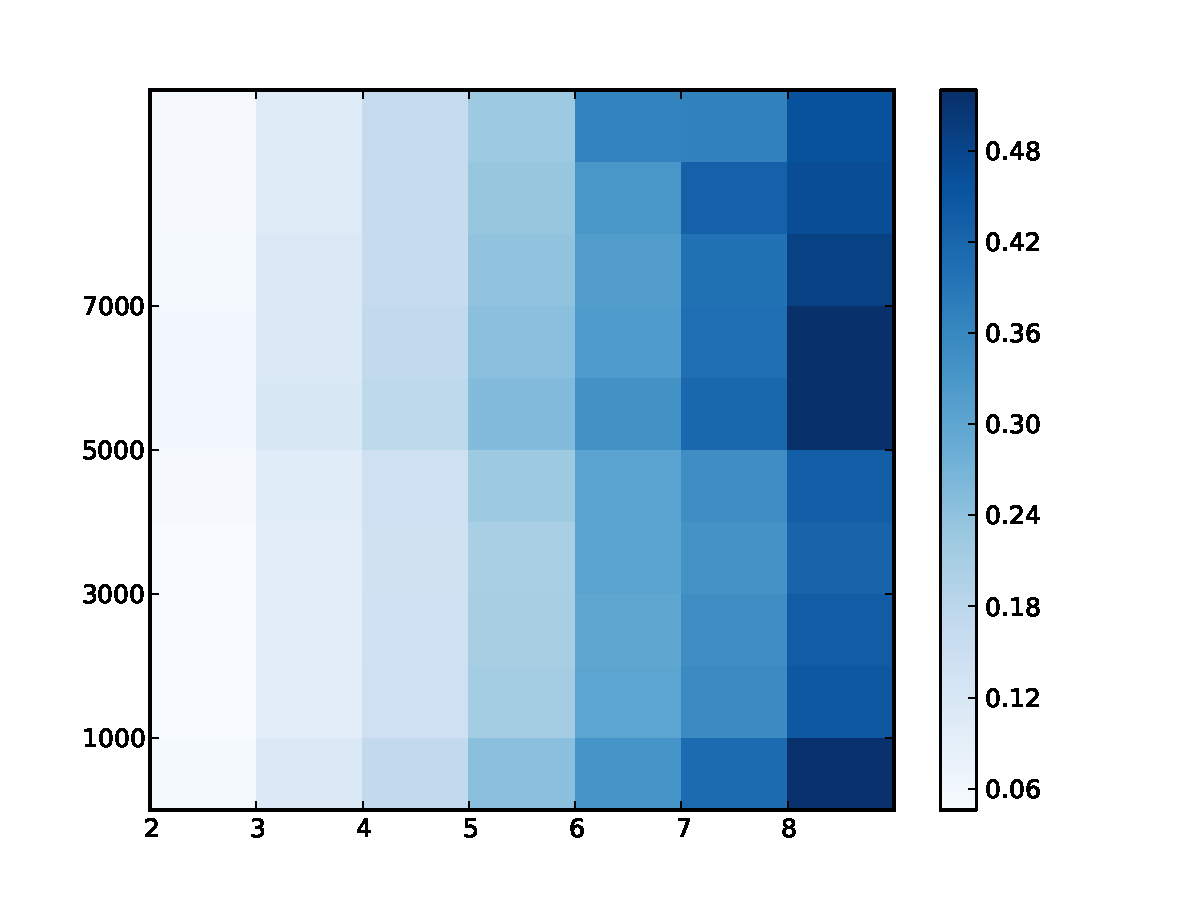
\includegraphics[width=1.0\textwidth]{./multiplication-by-omega.pdf}
\end{figure}

\end{frame}

\section{Elimination}

\begin{frame}[allowframebreaks]
\frametitle{PLE Decomposition}

\begin{tabular}{ll}
\begin{minipage}{0.4\textwidth}
\begin{center}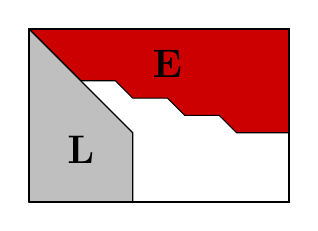
\begin{tikzpicture}[scale=0.22]
\draw[fill=white] (0,0) -- (0,10) -- (15,10) -- (15, 0) -- (0,0);
\draw[fill=red!80!black] (0,10) -- (3,7) -- (5,7) -- (6,6) -- (8,6) -- (9,5) -- (11,5) -- (12,4) -- (15,4) -- (15,10) -- (0,10);
\draw[fill=lightgray] (0,10) -- (6,4)  -- (6,0) -- (0,0) -- (0,10);

\draw[thick] (0,0) -- (0,10) -- (15,10) -- (15, 0) -- (0,0);
\node at (8,8) {\Large $\mathbf{E}$};
\node at (3,3) {\Large $\mathbf{L}$};
\end{tikzpicture}\end{center}
\end{minipage} & 
\begin{minipage}{0.5\textwidth}
\begin{definition}[PLE]
Let $A$ be a $m\times n$ matrix over a field $K$. A PLE decomposition of $A$ is
a triple of matrices $P,L$ and $E$ such that $P$ is a $m\times m$ permutation
matrix, $L$ is a unit lower triangular matrix, and $E$ is a $m\times n$ matrix
in row-echelon form, and $$A=PLE.$$
\end{definition}
\end{minipage}
\end{tabular}

\vspace{0.5cm}

PLE decomposition can be in-place, that is $L$ and $E$ are stored in $A$ and $P$ is stored as an $m$-vector.

\framebreak

From the PLE decomposition we can 
\begin{itemize}
 \item read the rank $r$,
 \item read the row rank profile (pivots),
 \item compute the null space,
 \item solve $y = Ax$ for $x$ and
 \item compute the (reduced) row echelon form.
\end{itemize}

\begin{thebibliography}{}
\bibitem{jeannerod-pernet-storjohann:cup2012}
C.-P. Jeannerod, C.~Pernet, and A.~Storjohann.
\newblock Rank-profile revealing {G}aussian elimination and the {CUP} matrix
  decomposition.
\newblock {\em {\tt arXiv:1112.5717}}, 35 pages, 2012.
 \end{thebibliography}


\end{frame}

\begin{frame}[allowframebreaks]
\frametitle{Block Recursive PLE Decomposition $\ord{n^{\omega}}$}

\vspace{-1.3em}
\begin{center}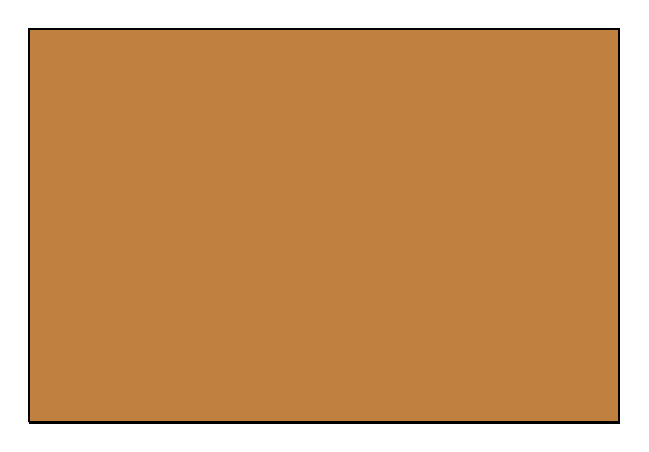
\begin{tikzpicture}[scale=0.5]
\draw[fill=brown] (0,0) -- (0,10) -- (15,10) -- (15, 0) -- (0,0);
\draw[thick] (0,0) -- (0,10) -- (15,10) -- (15, 0) -- (0,0);
\end{tikzpicture}\end{center}

\framebreak

\begin{center}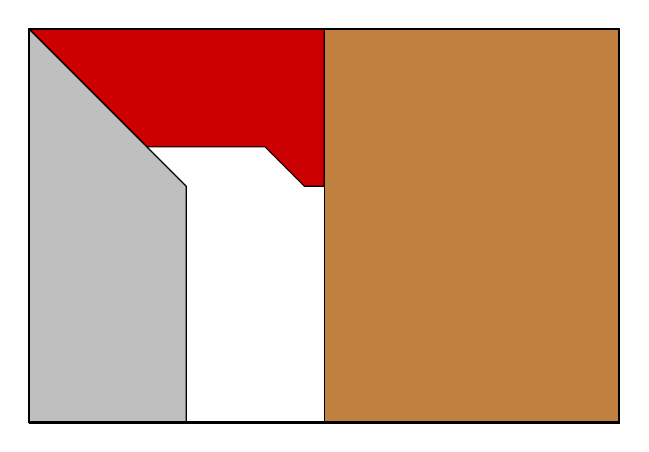
\begin{tikzpicture}[scale=0.5]
\draw[fill=brown] (0,0) -- (0,10) -- (15,10) -- (15, 0) -- (0,0);
\draw[fill=white] (0,0) --(0,10) -- (7.5,10) -- (7.5,0) -- (0,0);
\draw[fill=red!80!black] (0,10) -- (3,7) -- (6,7) -- (7,6) -- (7.5,6) -- (7.5,10) -- (0,10);
\draw[fill=lightgray] (0,10) -- (4,6) -- (4,0) -- (0,0) -- (0,10);
\draw[thick] (0,0) -- (0,10) -- (15,10) -- (15, 0) -- (0,0);
\end{tikzpicture}\end{center}

\framebreak

\begin{center}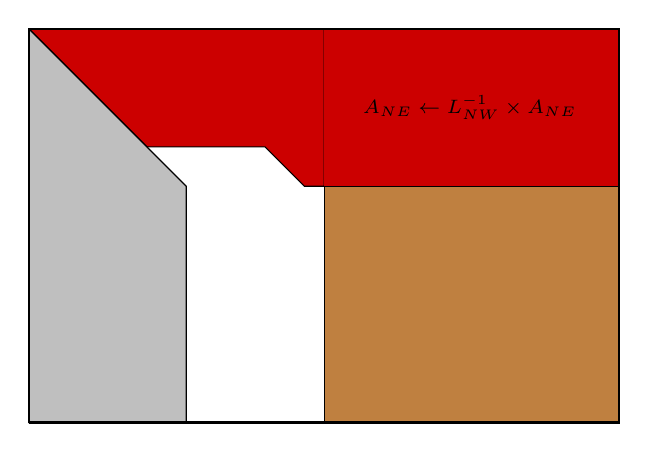
\begin{tikzpicture}[scale=0.5]
\draw[fill=brown] (0,0) -- (0,10) -- (15,10) -- (15, 0) -- (0,0);
\draw[fill=white] (0,0) --(0,10) -- (7.5,10) -- (7.5,0) -- (0,0);
\draw[fill=red!80!black] (0,10) -- (3,7) -- (6,7) -- (7,6) -- (7.5,6) -- (7.5,10) -- (0,10);
\draw[fill=lightgray] (0,10) -- (4,6) -- (4,0) -- (0,0) -- (0,10);
\draw[fill=red!80!black] (7.5,10) -- (15,10) -- (15,6) -- (7.5,6);
\node at (11.2,8) {\scriptsize $A_{NE} \leftarrow L_{NW}^{-1} \times A_{NE}$};
\draw[thick] (0,0) -- (0,10) -- (15,10) -- (15, 0) -- (0,0);
\end{tikzpicture}\end{center}

\framebreak

\begin{center}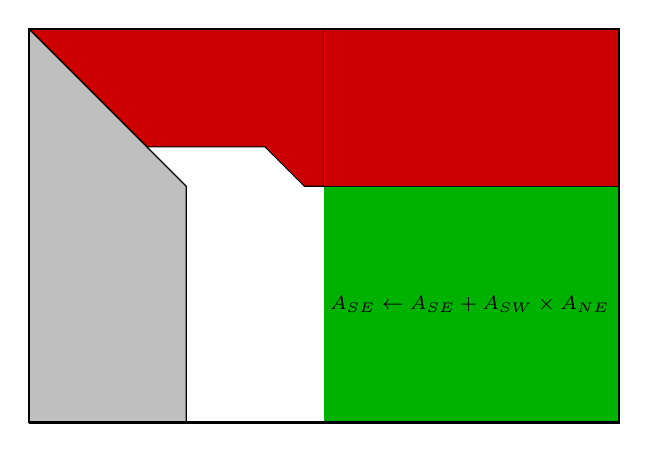
\begin{tikzpicture}[scale=0.5]
\draw[fill=brown] (0,0) -- (0,10) -- (15,10) -- (15, 0) -- (0,0);
\draw[fill=white] (0,0) --(0,10) -- (7.5,10) -- (7.5,0) -- (0,0);
\draw[fill=red!80!black] (0,10) -- (3,7) -- (6,7) -- (7,6) -- (7.5,6) -- (7.5,10) -- (0,10);
\draw[fill=lightgray] (0,10) -- (4,6) -- (4,0) -- (0,0) -- (0,10);
\draw[fill=red!80!black] (7.5,10) -- (15,10) -- (15,6) -- (7.5,6);
\draw[fill=green!70!black] (7.5,6) -- (15,6) -- (15,0) -- (7.5,0);
\node at (11.2,3) {\begin{scriptsize}$A_{SE} \leftarrow A_{SE} + A_{SW} \times A_{NE}$\end{scriptsize}};
\draw[thick] (0,0) -- (0,10) -- (15,10) -- (15, 0) -- (0,0);
\end{tikzpicture}\end{center}

\framebreak

\begin{center}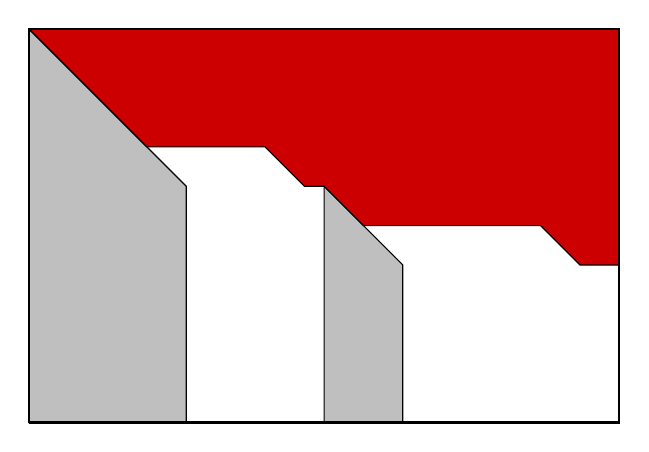
\begin{tikzpicture}[scale=0.5]
\draw[fill=white] (0,0) -- (0,10) -- (15,10) -- (15, 0) -- (0,0);
\draw[fill=lightgray] (0,10) -- (4,6) -- (4,0) -- (0,0) -- (0,10);
\draw[fill=lightgray] (7.5,6) -- (9.5,4) -- (9.5,0) -- (7.5,0) -- (7.5,6);
\draw[fill=red!80!black] (0,10) -- (3,7) -- (6,7) -- (7,6) -- (7.5,6) -- (8.5,5) -- (10,5) -- (13,5) -- (14,4) -- (15,4) -- (15,6) -- (15,10) -- (0,10);
\draw[thick] (0,0) -- (0,10) -- (15,10) -- (15, 0) -- (0,0);
\end{tikzpicture}\end{center}

\framebreak

\begin{center}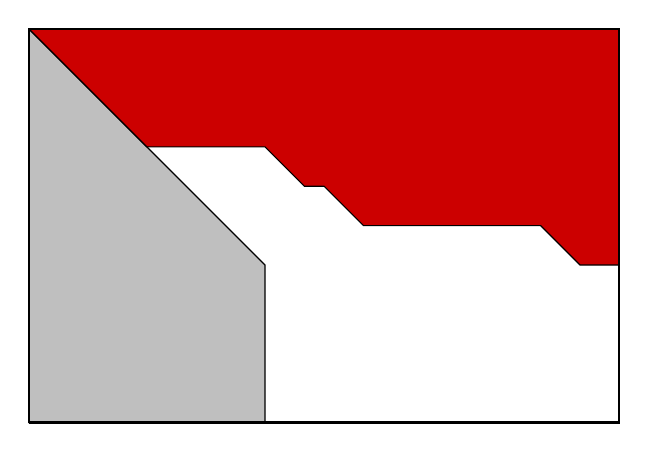
\begin{tikzpicture}[scale=0.5]
\draw[fill=white] (0,0) -- (0,10) -- (15,10) -- (15, 0) -- (0,0);
\draw[fill=lightgray] (0,10) -- (6,4) -- (6,0) -- (0,0) -- (0,10);
\draw[fill=red!80!black] (0,10) -- (3,7) -- (6,7) -- (7,6) -- (7.5,6) -- (8.5,5) -- (10,5) -- (13,5) -- (14,4) -- (15,4) -- (15,6) -- (15,10) -- (0,10);
\draw[thick] (0,0) -- (0,10) -- (15,10) -- (15, 0) -- (0,0);
\end{tikzpicture}\end{center}

\end{frame}

\begin{frame}
\frametitle{Ingredients} 

We need

\begin{enumerate}
 \item efficient matrix-matrix products ({\color{green}\bf DONE}),
 \item an efficient implementation of triangular system solving with matrices ({\color{orange}\bf NEXT}),
 \item an efficient PLE base case ({\color{orange}\bf NEXT}).
\end{enumerate}
\end{frame}

\begin{frame}[fragile]
\frametitle{Triangular System Solving}

\begin{columns}

\column{0.5\textwidth}

Triangular system solving with matrices also reduced to matrix-matrix multiplication, so all we need is an efficient base-case. 

\vspace{1em}

For that we use precomputation tables again.

\column{0.5\textwidth}

\begin{algorithm}[H]
\SetKw{KwContinue}{continue}
\SetKw{KwBreak}{break}
\Begin{
\For{$m > i \geq 0$}{
    $B_i \gets U_{i,i}^{-1} \cdot B_i$\;
    $T \gets$ \textsc{MakeTable}($B_i$)\;
    \For{$0 \leq j < i$} {
      $x \gets U_{j,i}$\;
      $B_j \gets B_j + T_x$\;
    }
}
}
\label{alg:travolta_trsm_upper_left}
\end{algorithm}
 
\end{columns}

\end{frame}


\begin{frame}
\frametitle{Gaussian elimination/PLE base case}

\begin{algorithm}[H]
\KwIn{$A$ -- $m \times n$ matrix}
\SetKw{KwContinue}{continue}
\Begin{
$r \longleftarrow 0$\;
\For{$0 \leq j < n$}{
  \For{$r \leq i < m$}{
   \lIf{$A_{i,j} = 0$} {
  \KwContinue\;
}
rescale row $i$ of $A$ such that $A_{i,j} = 1$\;
swap the rows $i$ and $r$ in $A$\;
$T \longleftarrow$ multiplication table for row $r$ of $A$\;
\For{$r+1 \leq k < m$} {
  $x \longleftarrow A_{k,j}$\;
  $A_k \longleftarrow A_k + T_x$\;
}
$r \longleftarrow r + 1$\;
  }
\Return{$r$}\;
}
}
\end{algorithm}
\end{frame}


\begin{frame}[allowframebreaks]
\frametitle{Results: Reduced Row Echelon Forms}
\begin{table}[ht]
\begin{small}
\begin{center}
\begin{tabular}{|r|r|r|r|r|r|}
\hline
 $e$ & Magma & GAP & LinBox & \multicolumn{2}{c|}{M4RIE}   \\
     & {\footnotesize 2.15-10} & {\footnotesize 4.4.12} & (mod $p$) 1.1.6 & \multicolumn{2}{c|}{\footnotesize 6b24b839a46f}\\
\hline
  2 &    6.04s &  162.65s & 49.52s &   3.31s & PLE\\
  3 &   14.47s &  442.52s & 49.92s &   5.33s & PLE\\
  4 &   60.37s &  502.67s & 50.91s &   6.33s & PLE\\
  5 &  659.03s &      N/A & 51.20s &  10.51s & PLE\\
  6 &  685.46s &      N/A & 51.61s &  13.08s & PLE\\
  7 &  671.88s &      N/A & 53.94s &  17.29s & PLE\\
  8 &  840.22s &      N/A & 64.24s &  20.25s & PLE\\
\hline
  9 & 1630.38s &      N/A & 76.18s & 260.77s & Gauss elim.\\
 10 & 1631.35s &      N/A & 76.45s & 291.30s & Gauss elim.\\
\hline
\end{tabular}
\end{center}
\end{small}
\caption{Elimination of $10,000 \times 10,000$ matrices on 2.66Ghz i7}
\label{tab:echelonform}
\end{table}


\begin{table}
\centering
\begin{scriptsize}
\begin{tabular}{|r||r|r|r|r|r|r|r|}
\hline
     & \multicolumn{7}{|c|}{CPU time in seconds}\\
\hline
$n$  & $e=2$ & $e=3$ & $e=4$ & $e=5$ & $e=6$ & $e=7$ & $e=8$\\
\hline
 1000 & 0.015 & 0.024 & 0.025 &  0.051 &  0.058 &  0.067 &  0.090\\
 2000 & 0.100 & 0.167 & 0.177 &  0.244 &  0.298 &  0.349 &  0.435\\
 3000 & 0.310 & 0.338 & 0.380 &  0.647 &  0.730 &  0.896 &  1.089\\
 4000 & 0.483 & 0.691 & 0.792 &  1.304 &  1.558 &  1.928 &  2.194\\
 5000 & 0.918 & 1.158 & 1.327 &  1.954 &  2.476 &  3.063 &  3.589\\
 6000 & 1.123 & 1.448 & 1.836 &  2.995 &  4.012 &  4.869 &  5.691\\
 7000 & 1.854 & 2.279 & 2.777 &  4.471 &  5.738 &  7.085 &  8.648\\
 8000 & 2.258 & 2.738 & 4.032 &  6.102 &  8.049 &  9.835 & 12.091\\
\hline
\hline
     & \multicolumn{7}{|c|}{CPU cycles / $n^{2.807}$}\\
\hline
$n$  & $e=2$ & $e=3$ & $e=4$ & $e=5$ & $e=6$ & $e=7$ & $e=8$\\
\hline
 1000 & 0.154 & 0.245 & 0.253 & 0.515 & 0.584 & 0.678 & 0.913\\
 2000 & 0.144 & 0.240 & 0.254 & 0.351 & 0.429 & 0.503 & 0.625\\
 3000 & 0.142 & 0.156 & 0.175 & 0.298 & 0.336 & 0.413 & 0.501\\
 4000 & 0.098 & 0.142 & 0.162 & 0.267 & 0.320 & 0.396 & 0.450\\
 5000 & 0.100 & 0.127 & 0.145 & 0.214 & 0.271 & 0.336 & 0.394\\
 6000 & 0.072 & 0.095 & 0.120 & 0.197 & 0.264 & 0.320 & 0.374\\
 7000 & 0.078 & 0.097 & 0.118 & 0.190 & 0.244 & 0.302 & 0.369\\
 8000 & 0.066 & 0.080 & 0.118 & 0.179 & 0.236 & 0.288 & 0.354\\
\hline
\end{tabular}
\end{scriptsize}
\caption{Gaussian elimination on \mycomputer}
\label{tab:moreelim}
\end{table}

\framebreak

\begin{figure}[h]
 \centering
 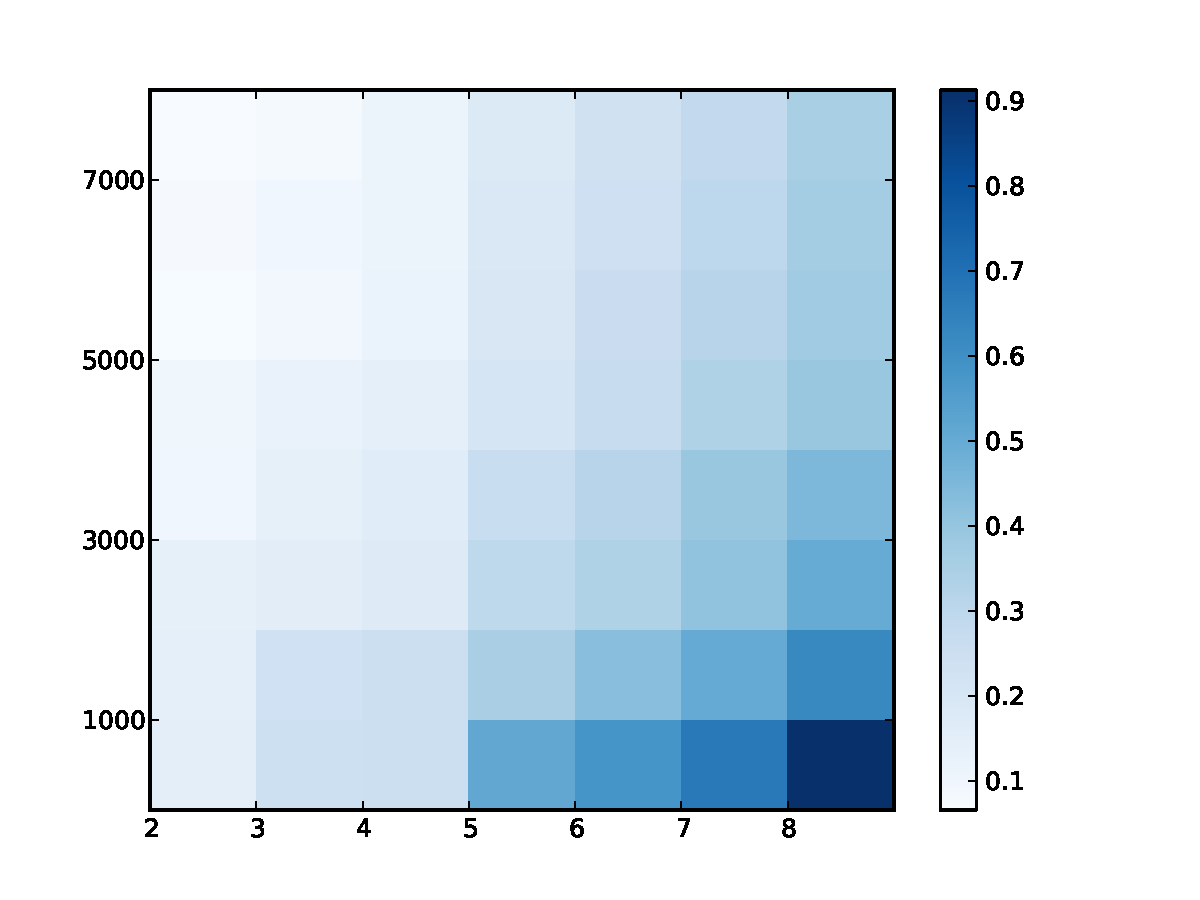
\includegraphics[width=1.0\textwidth]{./elimination-by-omega.pdf}
\end{figure}


\end{frame}


\begin{frame}[fragile]
\frametitle{Sensitivity to Sparsity}

\begin{figure}[htbp]
\begin{center}
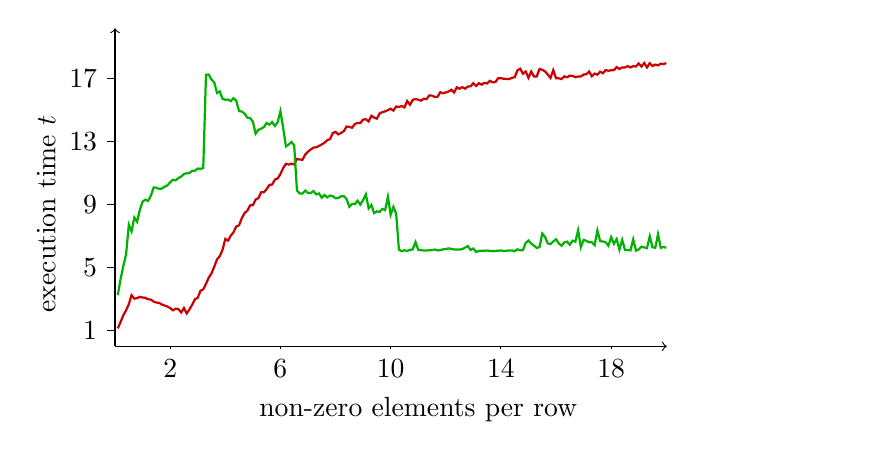
\begin{tikzpicture}[xscale=0.035,yscale=0.2]
  \draw[->] (-0.0,-0.0) -- (200.2,-0.0);
  \draw[->] (0,-0.0) -- (0,20.2);
  \draw (-25,8.4) node[rotate=90] {execution time $t$};

  \foreach \y in {1,5,...,20}
  \draw (0.1,\y) -- (-3,\y) node[anchor=east] {\y};

  %ticks
  \draw (20,-0.0) -- (20,-0.2) node[anchor=north] {2};
  \draw (60,-0.0) -- (60,-0.2) node[anchor=north] {6};
  \draw (100,-0.0) -- (100,-0.2) node[anchor=north] {10};
  \draw (140,-0.0) -- (140,-0.2) node[anchor=north] {14};
  \draw (180,-0.0) -- (180,-0.2) node[anchor=north] {18};

  \draw (110,-4.0) node {non-zero elements per row};

\draw[color=red!80!black,thick] plot[id="newtonjohn"] coordinates {
(  1.0,  1.14) (  2.0,  1.54) ( 3.0,   1.97) (  4.0,  2.29) (  5.0,  2.67) (  6.0,  3.25) (  7.0,  3.03) (  8.0,  3.06) (  9.0,  3.14) ( 10.0,  3.10) 
( 11.0,  3.08) ( 12.0,  2.99) ( 13.0,  2.97) ( 14.0,  2.84) ( 15.0,  2.78) ( 16.0,  2.76) ( 17.0,  2.65) ( 18.0,  2.59) ( 19.0,  2.53) ( 20.0,  2.43) 
( 21.0,  2.29) ( 22.0,  2.39) ( 23.0,  2.37) ( 24.0,  2.15) ( 25.0,  2.43) ( 26.0,  2.09) ( 27.0,  2.35) ( 28.0,  2.65) ( 29.0,  2.99) ( 30.0,  3.08) 
( 31.0,  3.53) ( 32.0,  3.62) ( 33.0,  3.97) ( 34.0,  4.37) ( 35.0,  4.63) ( 36.0,  5.06) ( 37.0,  5.52) ( 38.0,  5.73) ( 39.0,  6.13) ( 40.0,  6.82) 
( 41.0,  6.71) ( 42.0,  7.03) ( 43.0,  7.25) ( 44.0,  7.61) ( 45.0,  7.69) ( 46.0,  8.14) ( 47.0,  8.46) ( 48.0,  8.62) ( 49.0,  8.95) ( 50.0,  8.97) 
( 51.0,  9.32) ( 52.0,  9.41) ( 53.0,  9.78) ( 54.0,  9.78) ( 55.0,  9.98) ( 56.0, 10.25) ( 57.0, 10.27) ( 58.0, 10.59) ( 59.0, 10.66) ( 60.0, 10.94)
( 61.0, 11.32) ( 62.0, 11.59) ( 63.0, 11.54) ( 64.0, 11.60) ( 65.0, 11.55) ( 66.0, 11.90) ( 67.0, 11.86) ( 68.0, 11.85) ( 69.0, 12.18) ( 70.0, 12.36)
( 71.0, 12.50) ( 72.0, 12.62) ( 73.0, 12.64) ( 74.0, 12.72) ( 75.0, 12.82) ( 76.0, 12.93) ( 77.0, 13.09) ( 78.0, 13.16) ( 79.0, 13.54) ( 80.0, 13.62) 
( 81.0, 13.46) ( 82.0, 13.55) ( 83.0, 13.66) ( 84.0, 13.96) ( 85.0, 13.93) ( 86.0, 13.88) ( 87.0, 14.11) ( 88.0, 14.19) ( 89.0, 14.18) ( 90.0, 14.40) 
( 91.0, 14.42) ( 92.0, 14.28) ( 93.0, 14.64) ( 94.0, 14.53) ( 95.0, 14.46) ( 96.0, 14.79) ( 97.0, 14.87) ( 98.0, 14.92) ( 99.0, 15.00) (100.0, 15.09) 
(101.0, 14.97) (102.0, 15.23) (103.0, 15.20) (104.0, 15.26) (105.0, 15.17) (106.0, 15.58) (107.0, 15.34) (108.0, 15.65) (109.0, 15.70) (110.0, 15.66) 
(111.0, 15.60) (112.0, 15.72) (113.0, 15.70) (114.0, 15.93) (115.0, 15.92) (116.0, 15.84) (117.0, 15.84) (118.0, 16.14) (119.0, 16.07) (120.0, 16.12) 
(121.0, 16.18) (122.0, 16.29) (123.0, 16.12) (124.0, 16.45) (125.0, 16.36) (126.0, 16.46) (127.0, 16.36) (128.0, 16.50) (129.0, 16.51) (130.0, 16.71) 
(131.0, 16.53) (132.0, 16.71) (133.0, 16.62) (134.0, 16.73) (135.0, 16.69) (136.0, 16.86) (137.0, 16.77) (138.0, 16.78) (139.0, 17.03) (140.0, 17.03) 
(141.0, 16.99) (142.0, 16.98) (143.0, 16.97) (144.0, 17.05) (145.0, 17.09) (146.0, 17.53) (147.0, 17.63) (148.0, 17.31) (149.0, 17.45) (150.0, 17.05) 
(151.0, 17.45) (152.0, 17.14) (153.0, 17.14) (154.0, 17.61) (155.0, 17.56) (156.0, 17.46) (157.0, 17.26) (158.0, 17.04) (159.0, 17.54) (160.0, 17.02) 
(161.0, 17.02) (162.0, 16.97) (163.0, 17.14) (164.0, 17.09) (165.0, 17.19) (166.0, 17.17) (167.0, 17.09) (168.0, 17.13) (169.0, 17.14) (170.0, 17.26) 
(171.0, 17.28) (172.0, 17.45) (173.0, 17.15) (174.0, 17.32) (175.0, 17.25) (176.0, 17.44) (177.0, 17.34) (178.0, 17.54) (179.0, 17.50) (180.0, 17.53) 
(181.0, 17.54) (182.0, 17.73) (183.0, 17.61) (184.0, 17.71) (185.0, 17.71) (186.0, 17.80) (187.0, 17.71) (188.0, 17.79) (189.0, 17.77) (190.0, 17.96) 
(191.0, 17.77) (192.0, 17.99) (193.0, 17.71) (194.0, 17.98) (195.0, 17.80) (196.0, 17.89) (197.0, 17.84) (198.0, 17.95) (199.0, 17.92) (200.0, 17.99)
} node[right,color=white] {Newton-John};


\draw[color=green!70!black,thick] plot[id="ple"] coordinates {
(  1.0,  3.25) (  2.0, 4.27) (  3.0,  5.09) (  4.0,  5.84) (  5.0,  7.72) (  6.0,  7.30) (  7.0, 8.18) (  8.0,  7.91) (  9.0,  8.66) ( 10.0,  9.19)
( 11.0,  9.32) ( 12.0, 9.23) ( 13.0,  9.57) ( 14.0, 10.09) ( 15.0, 10.07) ( 16.0, 10.00) ( 17.0,10.02) ( 18.0, 10.14) ( 19.0, 10.22) ( 20.0, 10.42)
( 21.0, 10.58) ( 22.0,10.54) ( 23.0, 10.69) ( 24.0, 10.78) ( 25.0, 10.94) ( 26.0, 10.99) ( 27.0,11.00) ( 28.0, 11.15) ( 29.0, 11.15) ( 30.0, 11.29) 
( 31.0, 11.27) ( 32.0,11.32) ( 33.0, 17.25) ( 34.0, 17.26) ( 35.0, 16.94) ( 36.0, 16.76) ( 37.0,16.09) ( 38.0, 16.19) ( 39.0, 15.72) ( 40.0, 15.66) 
( 41.0, 15.67) ( 42.0,15.57) ( 43.0, 15.76) ( 44.0, 15.59) ( 45.0, 14.94) ( 46.0, 14.91) ( 47.0,14.78) ( 48.0, 14.52) ( 49.0, 14.50) ( 50.0, 14.27) 
( 51.0, 13.50) ( 52.0,13.75) ( 53.0, 13.82) ( 54.0, 13.92) ( 55.0, 14.18) ( 56.0, 14.08) ( 57.0,14.24) ( 58.0, 13.99) ( 59.0, 14.23) ( 60.0, 14.93)
( 61.0, 13.86) ( 62.0,12.70) ( 63.0, 12.81) ( 64.0, 12.98) ( 65.0, 12.76) ( 66.0,  9.90) ( 67.0, 9.70) ( 68.0,  9.70) ( 69.0,  9.89) ( 70.0,  9.74)
( 71.0,  9.74) ( 72.0, 9.86) ( 73.0,  9.65) ( 74.0,  9.71) ( 75.0,  9.44) ( 76.0,  9.61) ( 77.0, 9.46) ( 78.0,  9.58) ( 79.0,  9.53) ( 80.0,  9.40)
( 81.0,  9.42) ( 82.0, 9.52) ( 83.0,  9.54) ( 84.0,  9.36) ( 85.0,  8.86) ( 86.0,  9.04) ( 87.0, 9.03) ( 88.0,  9.25) ( 89.0,  9.00) ( 90.0,  9.28) 
( 91.0,  9.65) ( 92.0, 8.76) ( 93.0,  8.97) ( 94.0,  8.46) ( 95.0,  8.57) ( 96.0,  8.54) ( 97.0, 8.73) ( 98.0,  8.65) ( 99.0,  9.49) ( 100.0, 8.36) 
(101.0,  8.86) (102.0, 8.42) (103.0,  6.14) (104.0,  6.04) (105.0,  6.10) (106.0,  6.06) (107.0,  6.13) (108.0, 6.15) (109.0,  6.62) (110.0, 6.13)
(111.0,  6.10) (112.0, 6.09) (113.0,  6.09) (114.0,  6.10) (115.0,  6.11) (116.0,  6.15) (117.0, 6.09) (118.0,  6.11) (119.0,  6.16) (120.0,  6.18)
(121.0,  6.22) (122.0, 6.19) (123.0,  6.15) (124.0,  6.15) (125.0,  6.14) (126.0,  6.18) (127.0, 6.27) (128.0,  6.36) (129.0,  6.12) (130.0,  6.21)
(131.0,  5.99) (132.0,  6.06) (133.0,  6.07) (134.0, 6.07) (135.0,  6.08) (136.0,  6.07) (137.0, 6.04) (138.0,  6.06) (139.0,  6.07) (140.0,  6.09)
(141.0,  6.05) (142.0,  6.07) (143.0, 6.09) (144.0,  6.09) (145.0,  6.04) (146.0,  6.16) (147.0, 6.10) (148.0,  6.11) (149.0,  6.57) (150.0,  6.72)
(151.0,  6.52) (152.0, 6.39) (153.0,  6.25) (154.0,  6.30) (155.0,  7.16) (156.0,  6.95) (157.0, 6.53) (158.0,  6.50) (159.0,  6.66) (160.0,  6.80)
(161.0,  6.54) (162.0, 6.39) (163.0,  6.60) (164.0,  6.65) (165.0,  6.45) (166.0,  6.71) (167.0, 6.65) (168.0,  7.36) (169.0,  6.30) (170.0,  6.76)
(171.0,  6.70) (172.0, 6.61) (173.0,  6.61) (174.0,  6.42) (175.0,  7.36) (176.0,  6.68) (177.0, 6.66) (178.0,  6.61) (179.0,  6.39) (180.0,  6.94)
(181.0,  6.51) (182.0, 6.81) (183.0,  6.14) (184.0,  6.76) (185.0,  6.13) (186.0,  6.12) (187.0, 6.09) (188.0,  6.79) (189.0,  6.08) (190.0,  6.15)
(191.0,  6.33) (192.0, 6.28) (193.0,  6.24) (194.0,  6.99) (195.0,  6.29) (196.0,  6.26) (197.0, 7.12) (198.0,  6.25) (199.0,  6.31) (200.0,  6.26)
} node[right,color=white] {PLE};



\end{tikzpicture}
\caption{Gaussian elimination of $10,000 \times 10,000$ matrices over $\F_{16}$ on 2.67GHz Intel Core i7 M 620.}
\label{fig:sparse-m4rie}
\end{center}
\end{figure}
\end{frame}

\begin{frame}{Fin}
\begin{figure}[h]
 \centering
 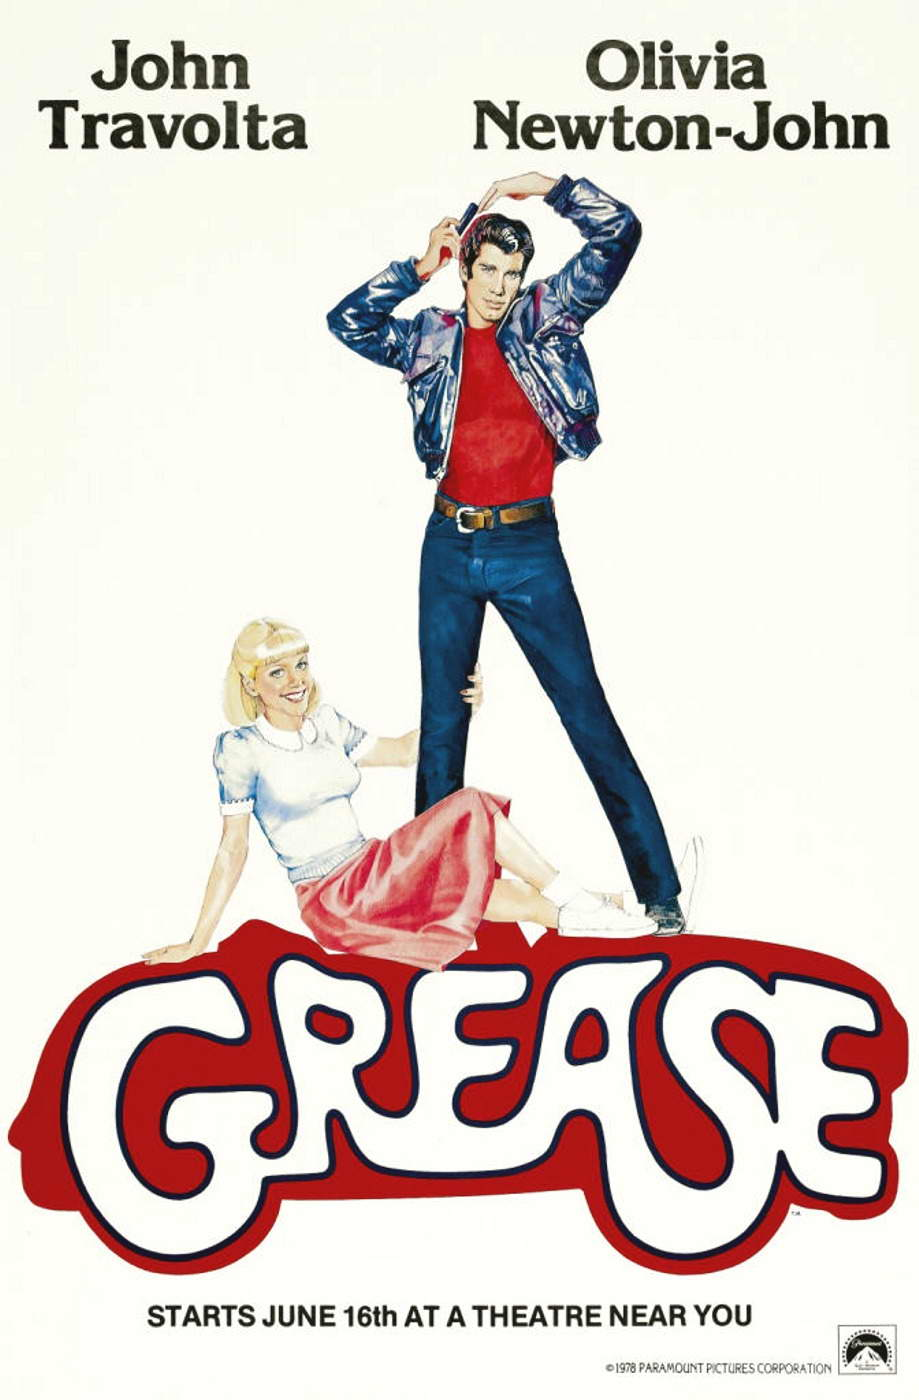
\includegraphics[width=0.4\textwidth]{./grease.jpg}
\end{figure}

\begin{center}

\end{center}

\end{frame}

\begin{frame}[allowframebreaks]
\bibliographystyle{alpha}
\bibliography{../../literature}
\end{frame}

\end{document}
